\chapter{Framework}\label{cap.framework}
This chapter serves as a way to introduce the tools that I have employed during the development of this project. All of them are \textbf{open-source}. The transparency provided by the open-source platforms is a major advantage because the software can be joined together and adapted to our specific application, which is mainly written in \textbf{Python} \footnote{\url{https://www.python.org/}}.

\section{JdeRobot}
\textbf{JdeRobot} \footnote{\url{http://jderobot.org}} is an open source middleware for robotics and computer vision. It has been designed to simplify the software development in these fields. It's mostly written in C++ language and it's structured like a collection of components (tools and drivers) that communicate to each other through \textbf{ICE interfaces} \footnote{\url{https://zeroc.com/products/ice}}. It is also compatible with \textbf{ROS} \footnote{\url{http://www.ros.org/}}, which allows us to use ROS nodes and JdeRobot components simultaneously. This flexibility makes it very useful for our application.
We're going to employ its \textit{cameraserver} driver to capture images from different video sources.

\subsection{\textit{cameraserver}}
According to JdeRobot documentation, this driver can serve both real cameras and video files. It interacts with other components thanks to the \textit{Camera} interface.

In order to use \textit{cameraserver}, we have to properly set its configuration file. These are the parameters that we must specify:
\begin{itemize}
    \item A network address where the server is going to be listening.
    \item Parameters related with the video stream: URI, framerate, image size, format.
\end{itemize}

\section{Keras}
As stated by \textbf{Keras} documentation \cite{chollet2015keras}: "Keras is a high-level neural network library, written in Python and capable of running on top of either TensorFlow or Theano". TensorFlow and Theano are open-source libraries for numerical computation optimized for GPU and CPU. Currently, I'm running Keras on top of \textbf{Theano} \footnote{\url{http://deeplearning.net/software/theano/index.html}} optimized for CPU.

Every neural network in Keras is defined as a \textit{model}. For those neural networks which can be built as a stack of layers, Keras provides the \textit{\textbf{Sequential model}} object. It is also possible to build more complex models with multiple outputs and shared layers using the Keras \textit{functional API}.

Implementing a neural network with Keras is very intuitive. We just have to declare a \textit{Sequential model}, add the desired layers to that model and train it. Besides that, we can preprocess the input data and monitorize what is happening while the model is being trained with several built-in functions. It's also possible to build those functions on our own and integrate them into the Keras workflow.

Keras library provides a function to read \textbf{HDF5} \footnote{\url{https://support.hdfgroup.org/HDF5/doc/H5.format.html}} datasets that can be used as inputs to the neural networks. It also saves the \textit{model} structure and weights into HDF5 files.

\section{Scikit-Learn}
\textbf{Scikit-Learn} \footnote{\url {http://scikit-learn.org/stable/index.html}} is a machine learning library that includes a wide variety of algorithms for clustering, regression and classification. It can be used during the whole machine learning process: preprocessing, training, model selection and evaluation.

We're going to employ Scikit-Learn functions to evaluate the neural networks that we have developed with Keras. Using a tool that is independent from Keras allows us to compare the results achieved by different neural network libraries (e.g. Keras and Caffe).

\section{Octave}
\textbf{GNU Octave} \footnote{\url{https://www.gnu.org/software/octave/}} is a scientific programming language compatible with Matlab. It provides powerful tools for plotting. We're going to use these tools to visualize the data collected with Scikit-Learn about the performance of our models. An example of a visualization using Octave can be seen in the figure \ref{figura:conf_mat}.
\begin{figure}
	\centering
	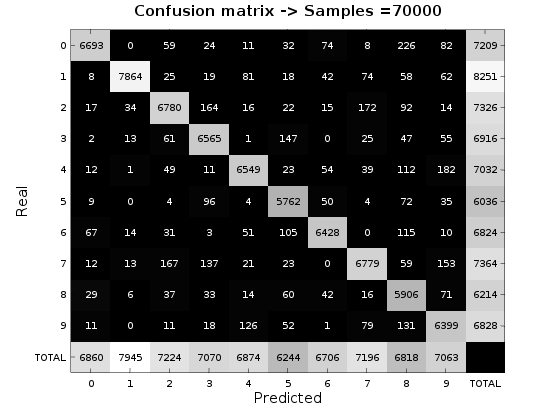
\includegraphics[width=12cm, keepaspectratio]{figures/conf_mat.png}
	\caption{Example of a confusion matrix visualization using Octave.}
	\label{figura:conf_mat}
\end{figure}